%%%%%%%%%%%%%%%%%%%%%%%%%%%%%%%%%%%%%%%%%%%%%%%%%%%%%%%%%%%
\section{Theory}
\label{sec:theory}
%%%%%%%%%%%%%%%%%%%%%%%%%%%%%%%%%%%%%%%%%%%%%%%%%%%%%%%%%%%
\subsection{Controlling covariance using friction}
Global inputs move a swarm uniformly.  
Controlling covariance requires breaking this uniform symmetry.  A swarm inside an axis-aligned rectangular workspace can reduce variance normal to a wall by simply pushing the swarm into the boundary. Directly controlling covariance by pushing the swarm into a boundary requires changing the boundary.  An obstacle in the lower-right corner is enough to generate positive covariance.  Generating both positive and negative covariance requires additional obstacles.  Requiring special obstacle configuration also makes covariance control dependent on the local environment. 
  Instead of pushing our robots directly into a wall, this paper examines an oblique approach, by using boundaries that generate friction with the robots.  These frictional forces are  sufficient to break the symmetry caused by uniform inputs.  Robots touching a wall have a negative friction force that opposes movement along the boundary, as shown in Eq.\ \eqref{eq:frictionmodel}.  This  causes robots along the boundary to slow down compared to robots in free-space. This enables covariance control using  boundaries with arbitrary orientations. 
  
 Let the control input be a vector force $\vec{F}$ with magnitude $F$ and orientation $\theta$.  The force of friction $F_f$ is
\begin{align}
N &= F \cos(\theta) \nonumber\\
F_f &= \begin{cases}  \mu_f N, &  \mu_f N < F \sin(\theta)  \label{eq:frictionmodel} \\ 
F \sin(\theta), & \text{else} \end{cases}  \\%\sign(F \sin(\theta) ) \cdot  \max(0, | F sin\theta |- |F_f|)
F_{forward} &=  F \sin(\theta) - F_f  \nonumber
\end{align}
 Fig.~\ref{fig:friction} shows the resultant forces on two robots when one is touching a wall. As illustrated, bot experiences different net forces although each receive the same inputs.
  For ease of analysis, the following algorithms assume $\mu$ is infinite and robots touching the wall are prevented from sliding along the wall.
This means that if one robot is touching the wall and another robot is free, if the control input is parallel or into the wall, the touching robot will not move. 
The next section shows how a system with friction model \eqref{eq:frictionmodel} and two walls are sufficient to arbitrarily position two robots. 
\begin{figure}[h]
\begin{center}
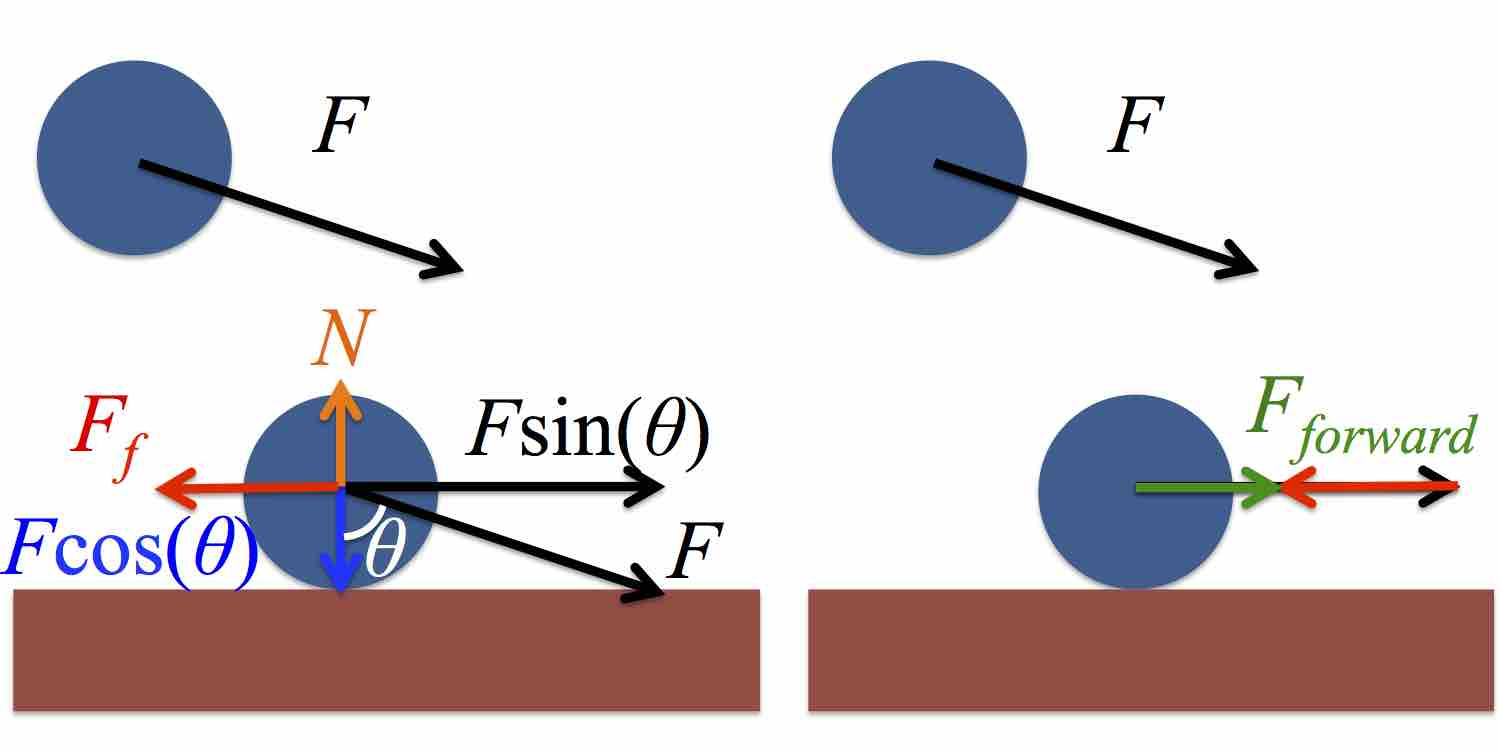
\includegraphics[width=\columnwidth/2]{friction.jpg} 
\caption{Wall friction reduces the force for going forward $F_{forward}$ on a robot near a wall, but not for a free robot.}
\label{fig:friction}
\end{center}
\end{figure} 




\section{Position control of $2$ robots using wall friction}\label{sec:PostionControl2Robots}
This section describes an algorithm for positioning two robots and introduces concepts that will be used for multi-robot positioning.
%Although the generalization of the proposed positioning algorithm in here is rather straightforward for multi robot systems, for the sake of simplicity we describe the algorithm designed for two robots. 
As we can see from Alg.~\ref{alg:PosControl2Robots}, assume two robots are initialized at $s_1$ and $s_2$ with corresponding goal destinations $e_1$ and $e_2$. 
Denote the current positions of the robots  $r_1$ and $r_2$. 
Let the subscripts $x$ and $y$ denote the $x$ and $y$ coordinates, i.e., $s_{1x}$ and $s_{1y}$ denote the $x$ and $y$ locations of $s_1$. 
The algorithm assigns a global control input at every instance.
 As a result, our goal is to adjust 
 $\Delta r_x = r_{2x}-r_{1x}$ from $\Delta s_x = s_{2x}-s_{1x}$ to $\Delta e_x = e_{2x}-e_{1x}$ and similarly adjust 
 $\Delta r_y = r_{2y}-r_{1y}$ from $\Delta s_y = s_{2y}-s_{1y}$ to $\Delta e_y = e_{2y}-e_{1y}$ with one global input at every instance. 
 The key to the algorithm is the position-dependent friction model \eqref{eq:frictionmodel}.
 %employing the assumption we have made earlier about the walls' friction. 

Our algorithm uses a divide and conquer method to solve the positioning problem. 
It finds the final position of the robots in two steps: (i) First, $|\Delta r_x - \Delta e_x |$ is reduced to zero while  $\Delta r_y$ is kept constant in Alg.~\ref{alg:XControl}. 
(ii) Having fixed $\Delta r_x$ to $\Delta e_x$ as desired, the  algorithm next keeps $\Delta r_x$ constant and adjusts $\Delta r_y$ to $\Delta e_y$, as desired in Alg..~\ref{alg:YControl}. 
Though steps (i) and (ii) are similar from an algorithmic point of view, the following subsections describe the process in detail. 

\subsection{Step (i): Fixing $\Delta r_x$}
\label{theory:step1}
\begin{itemize}
\item Define $e'_1=(e_{1x},s_{1y})$ and $e'_2=(e_{2x},s_{2y})$. Our goal for defining $e'_1$ and $e'_2$ is to understand the direction to which robots should move in order to adjust $\Delta r_x$. Let $e'_{\rm{top}} = \arg \max_i e'_{iy}$ and $e'_{\rm{bottom}} = \arg \min_i e'_{iy}$. Now if $e'_{\rm{top},x}-e'_{\rm{bottom},x}>0$, then the global input to both robots would be toward left direction and if $e'_{\rm{top},x}-e'_{\rm{bottom},x}<0$, then the global input to both robots would be toward right direction. The two robots continue their horizontal path until one of them reaches the $\epsilon$-neighborhood of one of the left or right walls.
\item At this step, let $y_{\min} = \min_i r_{iy}$, i.e., $y_{\min}$ is the minimum height of the two robots. We move both robots downward by the amount of $y_{\min}$ such that one of the robots would touch the bottom wall and hence friction force will not let that robot to move left or right.
\item The fact that the friction force of the bottom wall would not let the lower robot to move right or left will let the other robot to move to right and left freely to adjust $\Delta r_x $ according to $\Delta e_x$.
\item Finally, even if with the free move of the upper robot $\Delta r_x$ is not set to the $\Delta e_x$, we can run the Step (i) (as described in the previous paragraphs) again to adjust the $\Delta r_x$. It is easy to show that it is guaranteed that we can adjust $\Delta r_x$ to $\Delta e_x$ in only two iterations.
\end{itemize}

\subsection{Step (ii): Fixing $\Delta r_y$}
Now that we have adjusted the difference in robots' positions along one axis, we focus to do the same on the other axis as well. Therefore, similar to Section \ref{theory:step1}, we employ the following steps:
\begin{itemize}
\item Let $s'_1$ and $s'_2$ be the points we derived at the end of the steps in Section \ref{theory:step1}. 
\item Define $e''_1=(s'_{1x},e_{1y})$ and $e''_2=(s'_{2x},e_{2y})$. We define $e''_1$ and $e''_2$ to understand the direction to which robots should move in order to adjust $\Delta r_y$. Let $e''_{\rm{right}} = \arg \max_i e''_{ix}$ and $e''_{\rm{left}} = \arg \min_i e'_{ix}$. Now if $e''_{\rm{right},y}-e''_{\rm{left},y}>0$, then the global input to both robots would be toward down direction and if $e''_{\rm{right},y}-e''_{\rm{left},y}<0$, then the global input to both robots would be toward up direction. The two robots continue their vertical path until one of them reaches the $\epsilon$-neighborhood of one of the top or bottom walls.
\item At this step, let $x_{\min} = \min_i r_{ix}$, i.e., $x_{\min}$ is the minimum distance of the two robots from the origin along the $x$-axis. We move both robots to the left by the amount of $x_{\min}$ such that one of the robots would touch the left wall and hence friction force will not let that robot to move up or down.
\item The fact that the friction force of the left wall would not let one of the robots to move up or down will let the other robot to move to up or down freely to adjust $\Delta r_y $ according to $\Delta e_y$.
\item Finally, even if with the free move of the robot which is not touching the wall  $\Delta r_y$ is not set to the $\Delta e_y$, we can run the Step (i) (as described in the previous paragraphs) again to adjust the $\Delta r_y$. It is easy to show that it is guaranteed that we can adjust $\Delta r_y$ to $\Delta e_y$ in only two iterations.
\end{itemize}
Once $\Delta r_x$ and $\Delta r_y$ are set to $\Delta e_x$ and $\Delta e_y$, we can use global input to easily move both robots from $r_1$ and $r_2$ toward $e_1$ and $e_2$. 


\begin{algorithm}
\caption{WallFrictionArrange2Robots($s_1,s_2,e_1,e_2,L$)}\label{alg:PosControl2Robots}
\begin{algorithmic}[1]
\Require 
Knowledge of starting $(s_1,s_2)$ and ending $(e_1,e_2)$ positions of  two robots. 
$(0,0)$ is bottom corner, $s_1$ is rightmost robot, 
 $L$ is length of the walls. 
 Current position of the robots are $(r_1,r_2)$.

\State ($r_1,r_2$) = GenerateDesired$x$-spacing($s_1,s_2,e_1,e_2,L$)
\State GenerateDesired$y$-spacing($r_1,r_2,e_1,e_2,L$)

\end{algorithmic}
\end{algorithm}


\begin{algorithm}
\caption{GenerateDesired$x$-spacing($s_1,s_2,e_1,e_2,L$)}\label{alg:XControl}
\begin{algorithmic}[1]
\Require Knowledge of starting $(s_1,s_2)$ and ending $(e_1,e_2)$ positions of  two robots. 
$(0,0)$ is bottom corner, $s_1$ is topmost robot, 
 $L$ is length of the walls. Current robot positions are $(r_1,r_2)$.
\Ensure   $ r_{1y} - r_{2y}  \equiv s_{1y} - s_{2y} $   %$\Delta y(t) \equiv \Delta y(0)$ 
\State $\epsilon \gets $ small number
\State $ \Delta s_x  \gets s_{1x} - s_{2x} $
\State $ \Delta e_x \gets e_{1x} - e_{2x} $
\State $ r_1 \gets s_1$, $ r_2 \gets s_2$
\If {$\Delta e_x < 0 $ }
\State $ m \gets ( L-\epsilon-\max( r_{1x},r_{2x}) ,0)   $ \Comment{Move to right wall}
\Else 
\State  $ m \gets ( \epsilon-\min( r_{1x},r_{2x}),0 )    $ \Comment{Move to left wall}
\EndIf
\State $m  \gets  m + (0, -\min( r_{1y},r_{2y} ))$ \Comment{Move to bottom}
\State $ r_1 \gets r_1+m$, $ r_2 \gets r_2+m$ \Comment{Apply move}
\If {$\Delta e_x - (r_{1x} - r_{2x} ) > 0 $}
\State $ m \gets (\min(|\Delta e_x - \Delta s_x |, L- r_{1x}), 0)$  \Comment{Move right}
\Else
\State $ m \gets (-\min(|\Delta e_x - \Delta s_x |, r_{1x}), 0)$\Comment{Move left}
\EndIf 
\State $m  \gets  m + (0, \epsilon)$ \Comment{Move up}
\State $ r_1 \gets r_1+m$, $ r_2 \gets r_2+m$ \Comment{Apply move}
\State $\Delta r_x = r_{1x} - r_{2x}$
\If {$\Delta r_x \equiv \Delta e_x$} 
%\State   $ m \gets (e_{1x}-r_{1x}, e_{1y}-r_{1y})$
%\State $ r_1 \gets r_1+m$, $ r_2 \gets r_2+m$ \Comment{Apply move}
\State  \Return $(r_1,r_2)$
\Else   
\State \Return GenerateDesired$x$-spacing($r_1,r_2,e_1,e_2,L$)
\EndIf
\end{algorithmic}
\end{algorithm}

\begin{algorithm}
\caption{GenerateDesired$y$-spacing($s_1,s_2,e_1,e_2,L$)}\label{alg:YControl}
\begin{algorithmic}[1]
\Require Knowledge of starting $(s_1,s_2)$ and ending $(e_1,e_2)$ positions of  two robots. 
$(0,0)$ is bottom corner, $s_1$ is rightmost robot, 
 $L$ is length of the walls. Current position of the robots are $(r_1,r_2)$.
\Ensure   $ r_{1x} - r_{2x}  \equiv s_{1x} - s_{2x} $   %$\Delta y(t) \equiv \Delta y(0)$ 
\State $ \Delta s_y  \gets s_{1y} - s_{2y} $
\State $ \Delta e_y \gets e_{1y} - e_{2y} $
\State $ r_1 \gets s_1$, $ r_2 \gets s_2$
\If {$\Delta e_y < 0 $ }
\State $ m \gets ( L-\max( r_{1y},r_{2y}) ,0)   $ \Comment{Move to top wall}
\Else 
\State  $ m \gets ( -\min( r_{1y},r_{2y}),0 )    $ \Comment{Move to bottom wall}
\EndIf
\State $m  \gets  m + (0, -\min( r_{1x},r_{2x} ))$ \Comment{Move to left}
\State $ r_1 \gets r_1+m$, $ r_2 \gets r_2+m$ \Comment{Apply move}
\If {$\Delta e_y - (r_{1y} - r_{2y} ) > 0 $}
\State $ m \gets (\min(|\Delta e_y - \Delta s_y |, L- r_{1y}), 0)$  \Comment{Move top}
\Else
\State $ m \gets (-\min(|\Delta e_y - \Delta s_y |, r_{1y}), 0)$\Comment{Move bottom}
\EndIf 
\State $m  \gets  m + (0, \epsilon)$ \Comment{Move right}
\State $ r_1 \gets r_1+m$, $ r_2 \gets r_2+m$ \Comment{Apply move}
\State $\Delta r_y = r_{1y} - r_{2y}$
\If {$\Delta r_y \equiv \Delta e_y$} 
\State   $ m \gets (e_{1x}-r_{1x}, e_{1y}-r_{1y})$
\State $ r_1 \gets r_1+m$, $ r_2 \gets r_2+m$ \Comment{Apply move}
\State  \Return $(r_1,r_2)$
\Else   
\State \Return GenerateDesired$y$-spacing($r_1,r_2,e_1,e_2,L$)
\EndIf
\end{algorithmic}
\end{algorithm}






\section{Position Control of $n$ robots using wall friction}\label{sec:PostionControlnRobots}
Algorithm \ref{alg:PosControl2Robots}  can be extended to control the position of $n$ robots using wall friction under several constraints. The solution described here is an iterative procedure with $n$ loops. The $k$th loop moves the $k$th robot from staging zone to the desired position in a build zone. At the end the $k$th loop, robots 1 through $k$ are in their desired final configuration in the build zone, and robots $k+1$ to $n$ are in the staging zone.

Assume an open workspace with four axis-aligned walls with infinite friction.

\begin{figure}
\begin{center}
	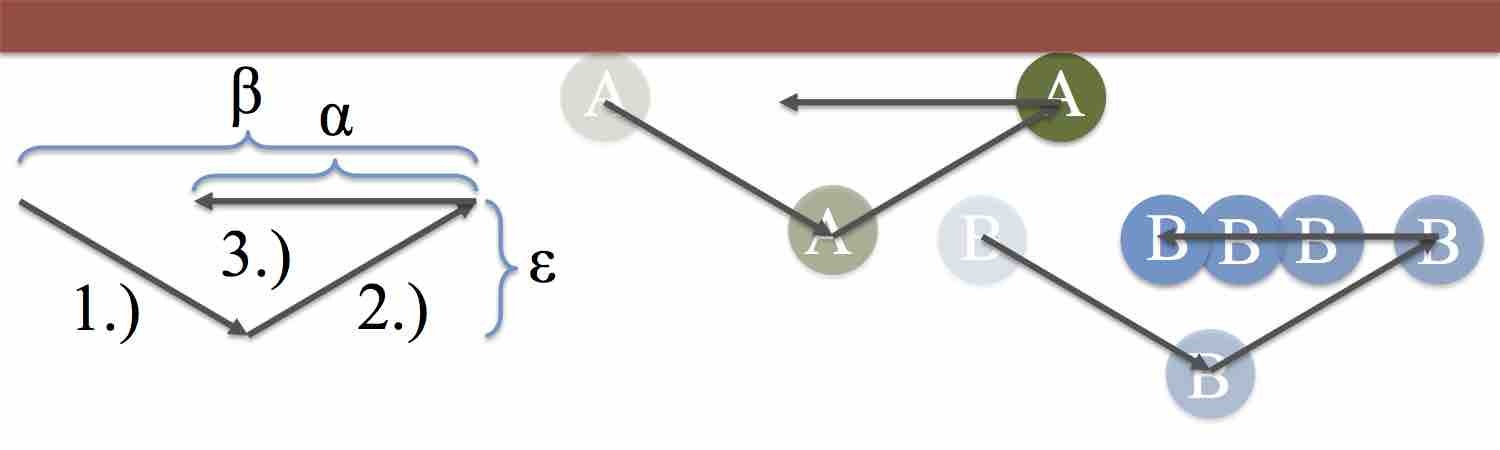
\includegraphics[width=1.0\columnwidth]{driftmove.jpg}
\end{center}
\caption{\label{fig:driftmove}
A  $\operatorname{DriftMove}(\alpha, \beta, \epsilon)$ consists of repeating a triangular movement sequence $\{ (\beta/2,-\epsilon),(\beta/2,\epsilon),(-\alpha,0)\}$. The robot $A$ touching a top wall will move right $\beta$ units, while robots not touching the top move right $\beta-\alpha$.
}
\end{figure}



The axis-aligned build zone of dimension $(w_b, h_b)$ containing the final configuration of $n$ robots must be disjoint from the axis-aligned staging zone of dimension $(w_s, h_s)$  containing the starting configuration of $n$ robots. Without loss of generality, assume the build zone  is above the staging zone . 
Furthermore, there must be at least $\epsilon$ space above the build zone, $\epsilon$ below the staging zone , and $\epsilon + 2r$ to the left of the build and staging zone, where $r$ is the radius of a robot.  The minimum workspace is then $(\epsilon + 2r + \max(w_f,w_s), 2\epsilon + h_s,h_f)$.

The $n$ robot position control algorithm relies on a $\operatorname{DriftMove}(\alpha, \beta, \epsilon)$ control input, shown in Fig.\  \ref{fig:driftmove}.
A drift move consists of repeating a triangular movement sequence $\{ (\beta/2,-\epsilon),(\beta/2,\epsilon),(-\alpha,0)\}$. The robot $A$ touching a top wall moves right $\beta$ units, while robots not touching the top move right $\beta-\alpha$.

Let $(0,0)$ be the lower left corner of the workspace, $p_k$ the $x,y$ position of the $k$th robot, and $f_k$ the final $x,y$ position of the $k$th robot. Label the robots in the staging zone from left-to-right and top-to-bottom, and the $f_k$ configurations right-to-left and top-to-bottom as shown in Fig.~\ref{fig:construction2d}.

\begin{algorithm}
\caption{PositionControl$n$RobotsUsingWallFriction($k$)}\label{alg:PosControlNRobots}
\begin{algorithmic}[1]
\State move( $-\epsilon, r-p_{k,y}$) % move  away from right wall and down till robot k touches bottom


\While{ $p_{k,x} > r$} 
\State $\operatorname{DriftMove}(0, \min(p_{k,x} - r,\epsilon), \epsilon)$ left   %drift move left until kth robot touches left wall
\EndWhile

\State $m \gets \operatorname{ceil}\frac{f_{ky}-r}{\epsilon}$
\State $\beta \gets \frac{f_{ky}-r}{m}$
\State $\alpha \gets \beta - \frac{\epsilon}{m}$
\For{ $m$ iterations}
\State $\operatorname{DriftMove}(\alpha, \beta, \epsilon)$ up   %move kth robot to f_{ky} and leave the rest in position.
\EndFor

\State move($r+\epsilon-f_{kx}, 0$)  % move the group to the left until k is in the correct relative x position
\State move($f_{kx}-r, 0$)  

\end{algorithmic}
\end{algorithm}
Algorithm \ref{alg:PosControlNRobots} procedes as follows:  
First, the robots are moved  away from right wall and down so robot $k$ touches bottom.
Second, a set of $\operatorname{DriftMove()}$s are executed that  move the $k$ robot to the left wall with no net movement on the other robots.
Third, a set of $\operatorname{DriftMove()}$s are executed that  move the $k$ robot to it's target height and return the other robots to their initial heights. 
Fourth, all robots except the $k$ robot are pushed left until the $k$ robot is in the correct relative $x$ position compared to robots 1 to $k-1$.
Finally, all robots are moved right until robot $k$ is in the desired target position.
\begin{figure}
\begin{center}
	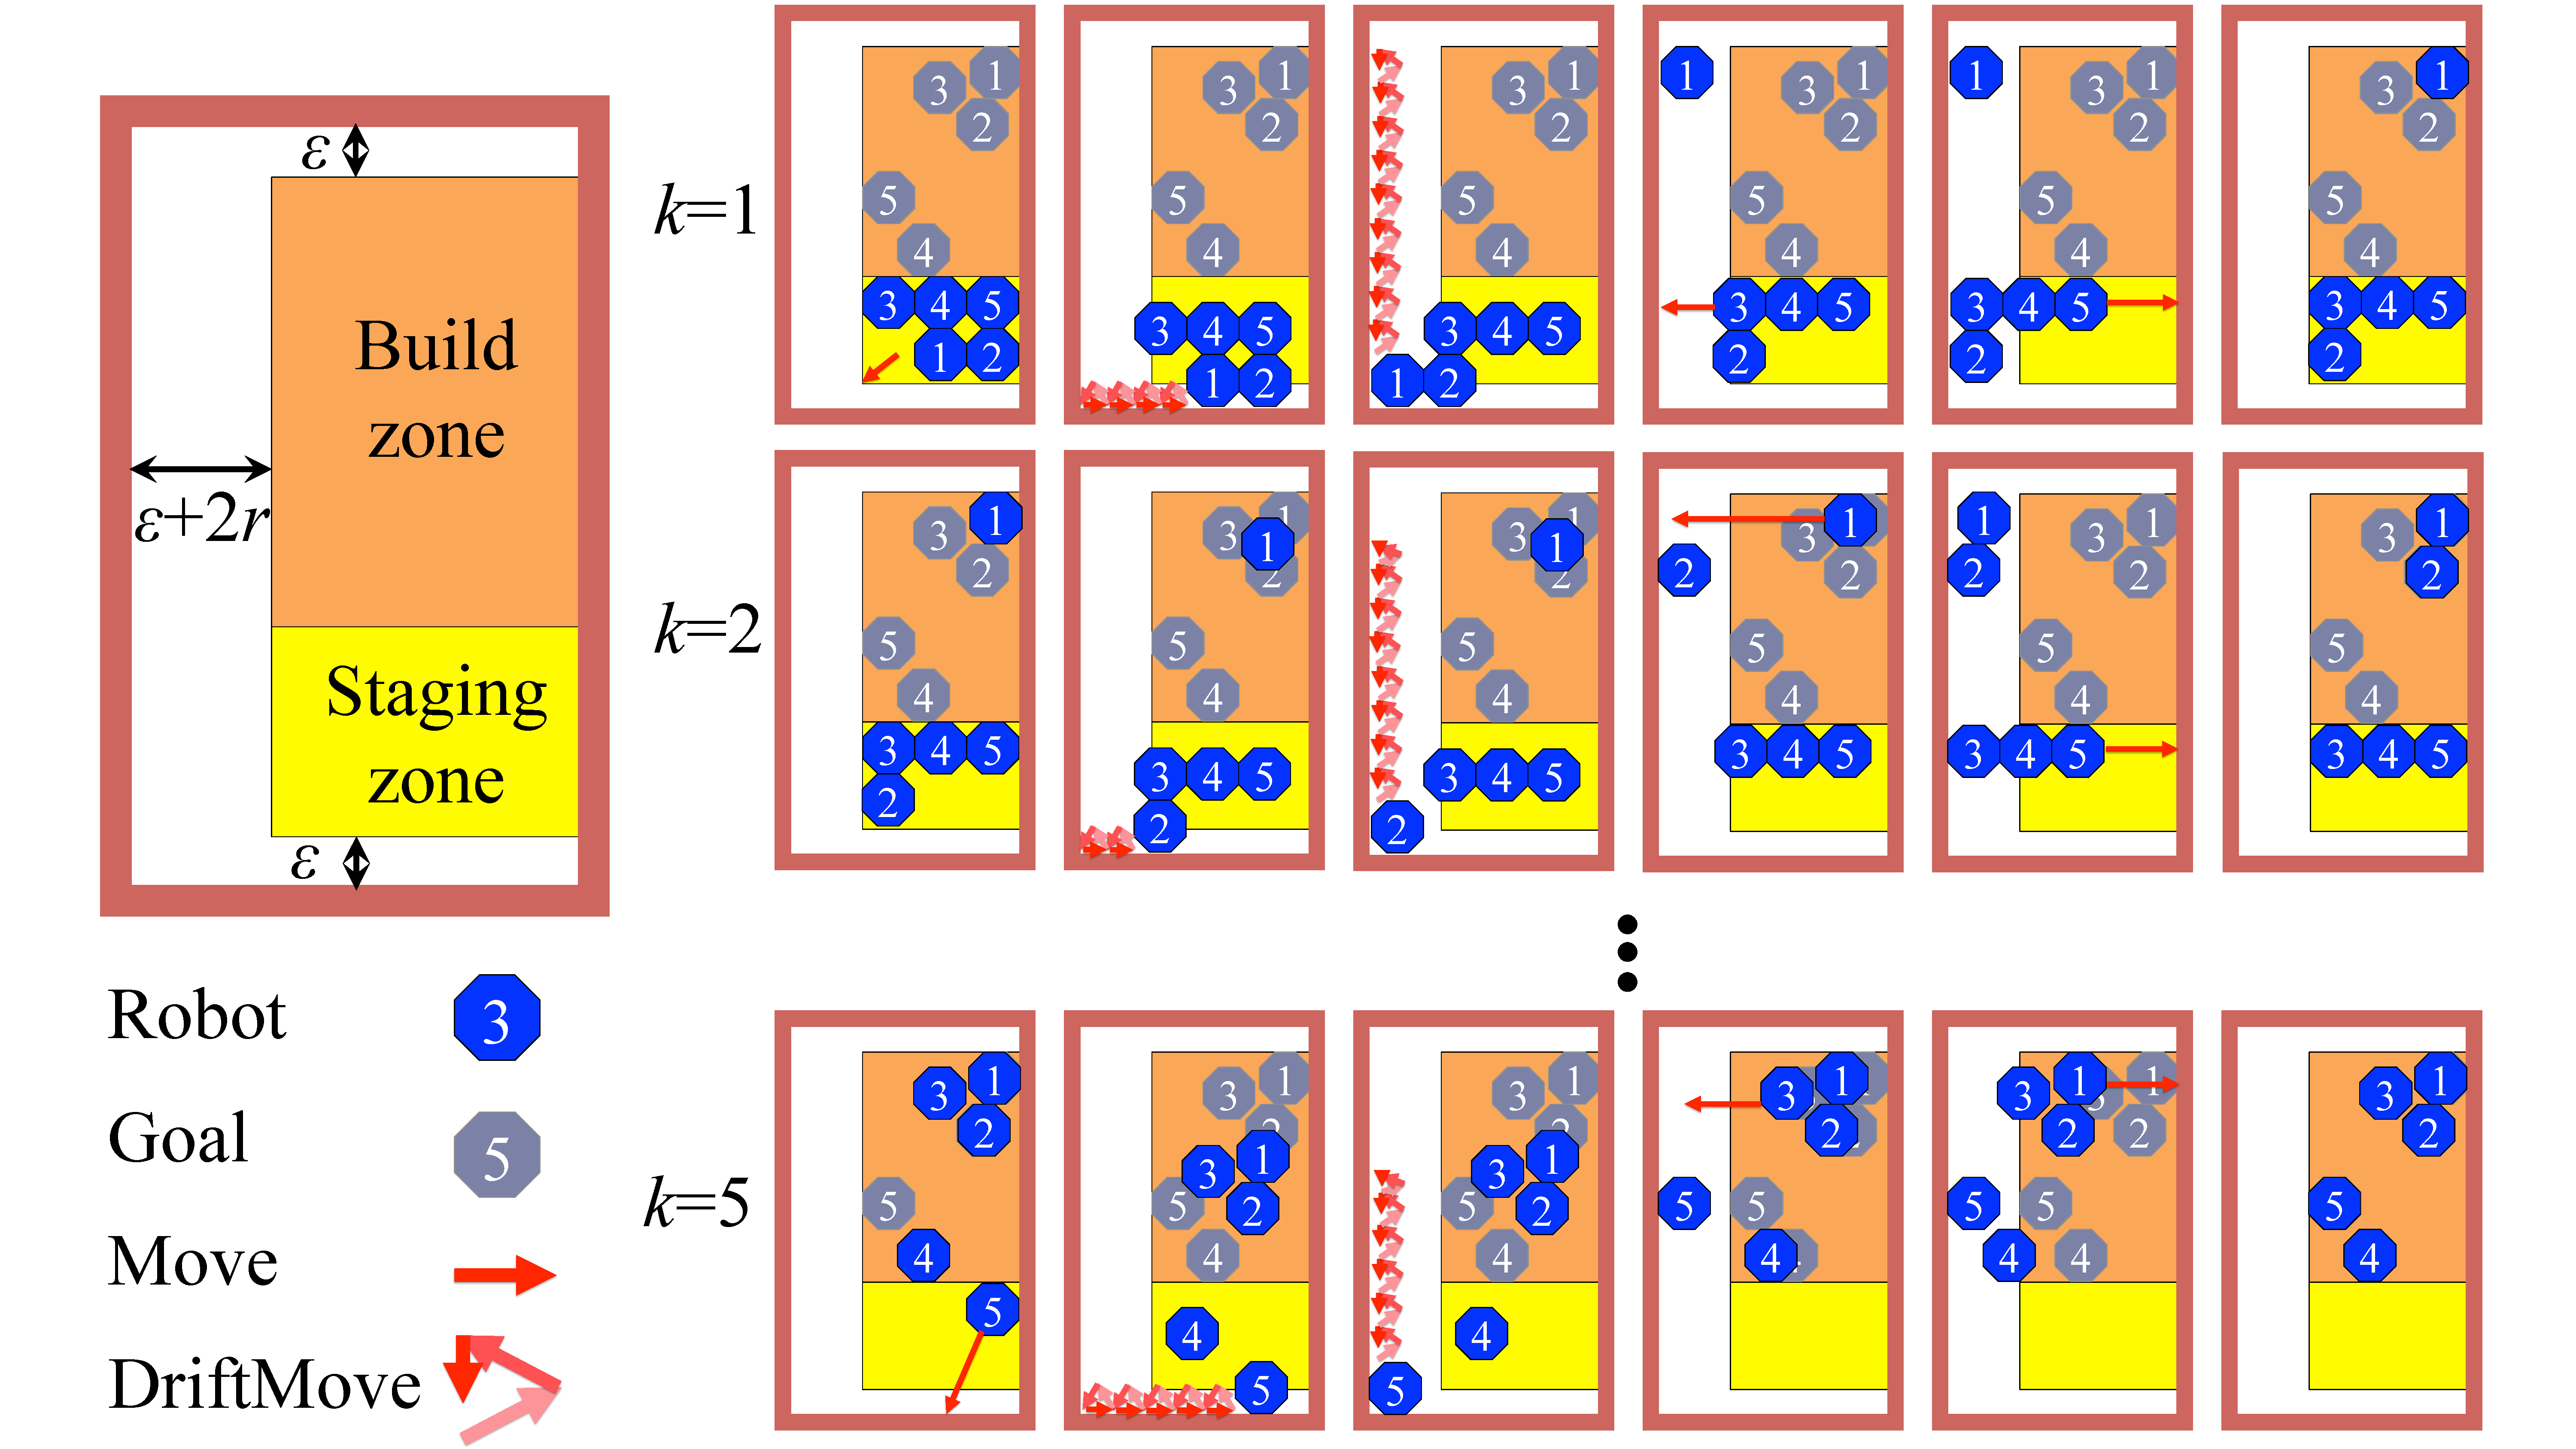
\includegraphics[width=1.0\columnwidth]{PositionNrobots.pdf}
\end{center}
\caption{\label{fig:construction2d}
Illustration of Alg.\ \ref{alg:PosControlNRobots}, $n$ robot position control  using wall friction.
}
\end{figure}













